%----------------------------------------------------------------------------------------
%	Part2 - 58Ghz attenuation
%----------------------------------------------------------------------------------------
\newpage

\section{Part2 - 58Ghz attenuation}
From 8 to 14 week I worked for Space technology laboratory supervised by Dr. László Csurgai-Horváth.
Our topic is to research about oxygen and rain attenuation on 58GHz radio signal.

\subsection{Introduction on 58GHz band}
Signal around 60Ghz band has a unique advantage. Around this frequency
signal propagation is effected by oxygen molecule in the air. This phenomenon is 
called oxygen attenuation. Because such phenomenon, signal can not propagate for long distance.
In urban area where high bandwidth communication is required this property can increse
frequency reuse rate which will conserve frequency band resource.

\subsection{Experiment setup}
Two antennas are placed on the roof of building V1 and building E.
An indoor unite was set in the laboratory for data logging.

\paragraph{Geometry}
Geolocation of antennas are measured using GPS coordinate where distance and
elevation angle can be calculated.
GPS coordinates are:
\begin{itemize}
    \item Building V1 antenna: 47.476647, 19.056420, 123.2m
    \item building E antenna: 47.477423, 19.057490, 146.8m
\end{itemize}

From above data we calculated distance $d = 118.0m$ 
and elevation angle $\theta = 11.537^\circ$

\paragraph{Hardware specification}
Testing divices are consist of indoor and outdoor units. Both manufactured by 
Nokia Network. Hardware specification are 
defined in the user manual of these units \cite{metrohopper}
\begin{itemize}
    \item Frequency: 57.725GHz
    \item Polarization: vertical
    \item Antenna gain: 34dB
    \item Transmitter output power: 5dBm
\end{itemize}

\newpage
\subsection{Calculations}
\paragraph{Free space loss}
Free space loss is the loss when signal travels through open space with no
other attenuation. This can be calculated using following equation \cite{openspace}

\begin{equation}
    a_{sz}^{[dB]} = 32.44 + 20log f^{[MHz]}+20log d^{[km]} - G_{TX}^{[dB]} - G_{RX}^{[dB]}
    \label{eq:openspace}
\end{equation}

Where:
\begin{itemize}
    \item $a_{sz}$ is free space loss in dB
    \item $f$ is radio frequency in MHz
    \item $d$ is distance between transmitter and receiver in km 
    \item $G_{TX}$ is transistor antenna gain in dB
    \item $G_{RX}$ is receiver antenna gain in dB
\end{itemize}
\paragraph{Oxygen attenuation}
Oxygen attenuation or Atmospheric attenuation is the effect of signal propagation due to
gas in the atmosphere. The following figure is given in ITU-R P.676 \cite{oxygen} which
demonstrate signal attenuation with different frequency. A peak at around 60GHz is 
clearly visiable which is casued by oxygen molecule in the air.

\begin{figure}[h!]
    \centering
    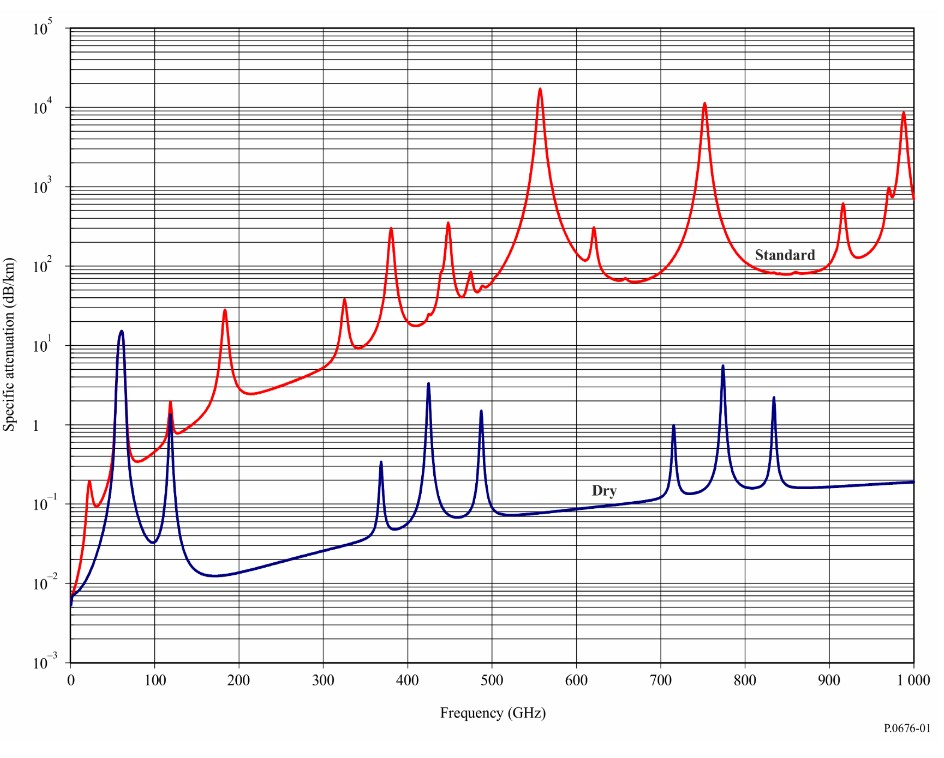
\includegraphics[width=0.9\linewidth]{oxygen.jpg}
    \caption{Atmospheric attenuation}
    \label{fig:Atmospheric attenuation}
\end{figure}

Calculations for oxygen attenuation is quit complicated but for estimation 
purpose Matlab provided a built-in function \verb|gaspl|

\begin{lstlisting}[language=Matlab]
    L = gaspl(range,freq,T,P,den)
\end{lstlisting}
arguments:
\begin{itemize}
    \item range: Signal path length in multimeters
    \item freq: Signal frequency in Hz
    \item T: Ambient temperature in degrees Celsius
    \item P: Dry air pressure in Pa 
    \item den: Water vapor density or absolute humidity in $g/m^3$
\end{itemize}

\paragraph{Rain attenuation}
Rain attenuation is our main research direction. We want to measure how
rain will effect signal propagation on this particular frequency.